\documentclass[Japanese]{dicomopapers}
%\documentclass[Japanese,noauthor]{dicomopapers}
\usepackage[dvips]{graphicx}
\usepackage{latexsym}

\def\Underline{\setbox0\hbox\bgroup\let\\\endUnderline}
\def\endUnderline{\vphantom{y}\egroup\smash{\underline{\box0}}\\}
\def\|{\verb|}

%概要投稿用余白調整ここから
\setlength{\Jauthorjreceivesep}{0.0mm}
\setlength{\Jreceivejabstsep}{0.0mm}
\setlength{\Jabstsepjkeyword}{0.0mm}
\setlength{\Jkeywordetitle}{0.0mm}
%概要投稿用余白調整ここまで

\begin{document}

% 和文表題
\title{SDNによる仮想デバイスを用いた\\セキュアなホームネットワーク内通信の検討}

% 英文表題
\etitle{Investigation of Secure Communication within a Home Network\\Using Virtual Devices with SDN}

% 所属ラベルの定義
\affiliate{DOSHISHA}{同志社大学大学院 理工学研究科\\Graduate School of Science and Engineering, Doshisha University}
\affiliate{MOBILITY}{同志社大学モビリティ研究センター\\Mobility Reserch Center, Doshisha University}

\author{塚崎 拓真}{TAKUMA TSUKASAKI}{DOSHISHA}
\author{滕 睿}{RUI TENG}{MOBILITY}
\author{佐藤 健哉}{KENYA SATO}{DOSHISHA}

% 表題などの出力
\maketitle

% 本文はここから始まる
\section{概要}
近年,IoT(Internet of Things)が注目を集めるようになり,今後あらゆるモノがネットワークに接続され,利用されることが予想される.\par
しかし,IoTの発展により利便性が高まる一方で,これまでネットワークに接続されていなかったモノが接続されることにより,セキュリティ上のリスクも高まっている.
IoTデバイスは十分なセキュリティを考慮せずに開発されたものが多いため,悪意のある攻撃者によるサイバー攻撃の標的になりやすい.
また,現在のスマートホームデバイスは,クラウド上のシステムと連携することで,デバイス間の連携を可能にしているが,今後はホームネットワーク内で閉じたデバイス間の通信によって連携を行う形になることが想定される.
デバイス間で直接通信を行う場合,各デバイスにおいてどのデバイスとの通信を受け入れるか,アクセス制御を行う必要がある.
% セキュリティ上の脅威が各種デバイスに顕在した場合,個別に対処するとコストや時間がかかってしまうため,脅威に対し一括に対処する必要がある.\par
% しかし,ホームネットワーク内には異なる規格のハードウェアや様々なアプリケーションが混在しているため,それら全てに対応したシステムの構築や更新を続けるのは困難である.
しかし,全てのデバイスがアクセス制御に対応しているとは限らず,デバイスの計算能力の制限によって実現できるアクセス制御に制限がある場合や,デバイスのソフトウェア自体の脆弱性によってアクセス制御が機能しない場合が考えられる.
そのため,ホームネットワーク内で通信するのであれば,どのデバイスも必ず利用するネットワークを利用したシステムを構築することが望ましい.\par
そこで本研究では,SDN(Software Defined Networks)の代表的プロトコルであるOpenFlowを用いて,ホームネットワークに適した形での不正な通信の検知を検討した.
% OpenFlowを利用することで,既存IoTデバイスや異なる規格などに対応でき,ホームネットワークに適した形で不正な通信の検知を実現する.
仮想デバイスというセキュリティ対策を適用可能なデバイスを,ルータ上に仮想的に作成する.
ここにIoTデバイスがリソースの都合上適用できないセキュリティ対策をオフロードし,この仮想デバイスがIoTデバイスの通信を中継し,仮想デバイス間通信も可能にすることで,本来IoTデバイスに適用したいセキュリティ対策を実現する.
セキュリティ対策として,ホームネットワーク内の通信のトラフィック情報は既知であることを考慮し,フローの検証をOpenFlowコントローラで行う.\par
ルータ内に仮想デバイスとしてOpenFlowスイッチを設置し,IoTデバイス間で閉じた通信を行うシミュレーションを実装し,ホームネットワークにおいてセキュリティ要件を保つことを示した.

\begin{figure}[!tb]
      \centering
      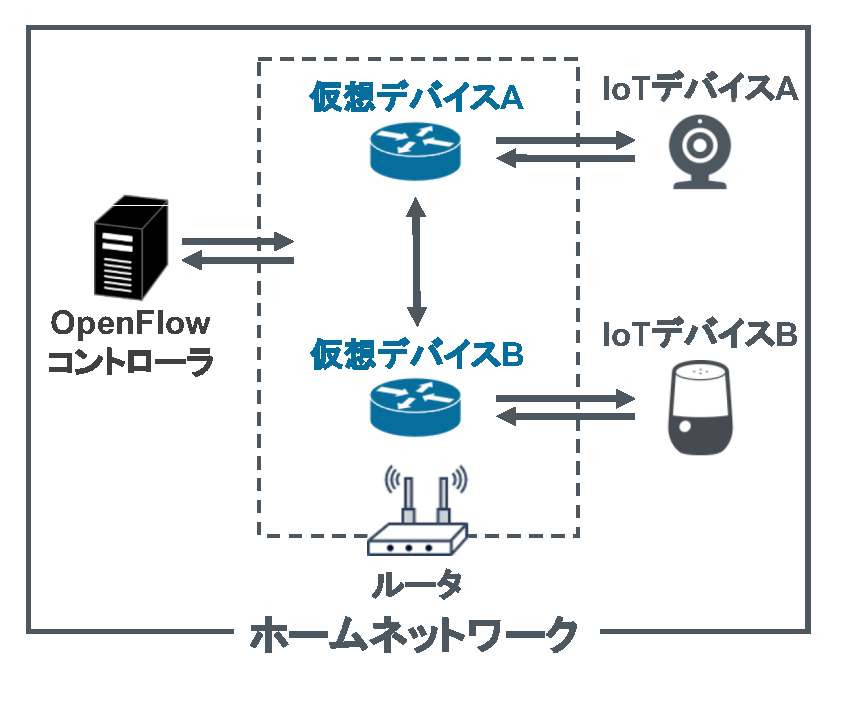
\includegraphics[width=\linewidth]{img/system.eps}
      \caption{提案手法の構成}
      \label{fig:syste}
\end{figure}

\end{document}
